\chapter*{Appendix}
\addcontentsline{toc}{part}{Appendix}
\label{sec:appendix}

\chapter{Quality control}
\section{Genotyping}

\begin{figure}[hbtp]
	\centering
	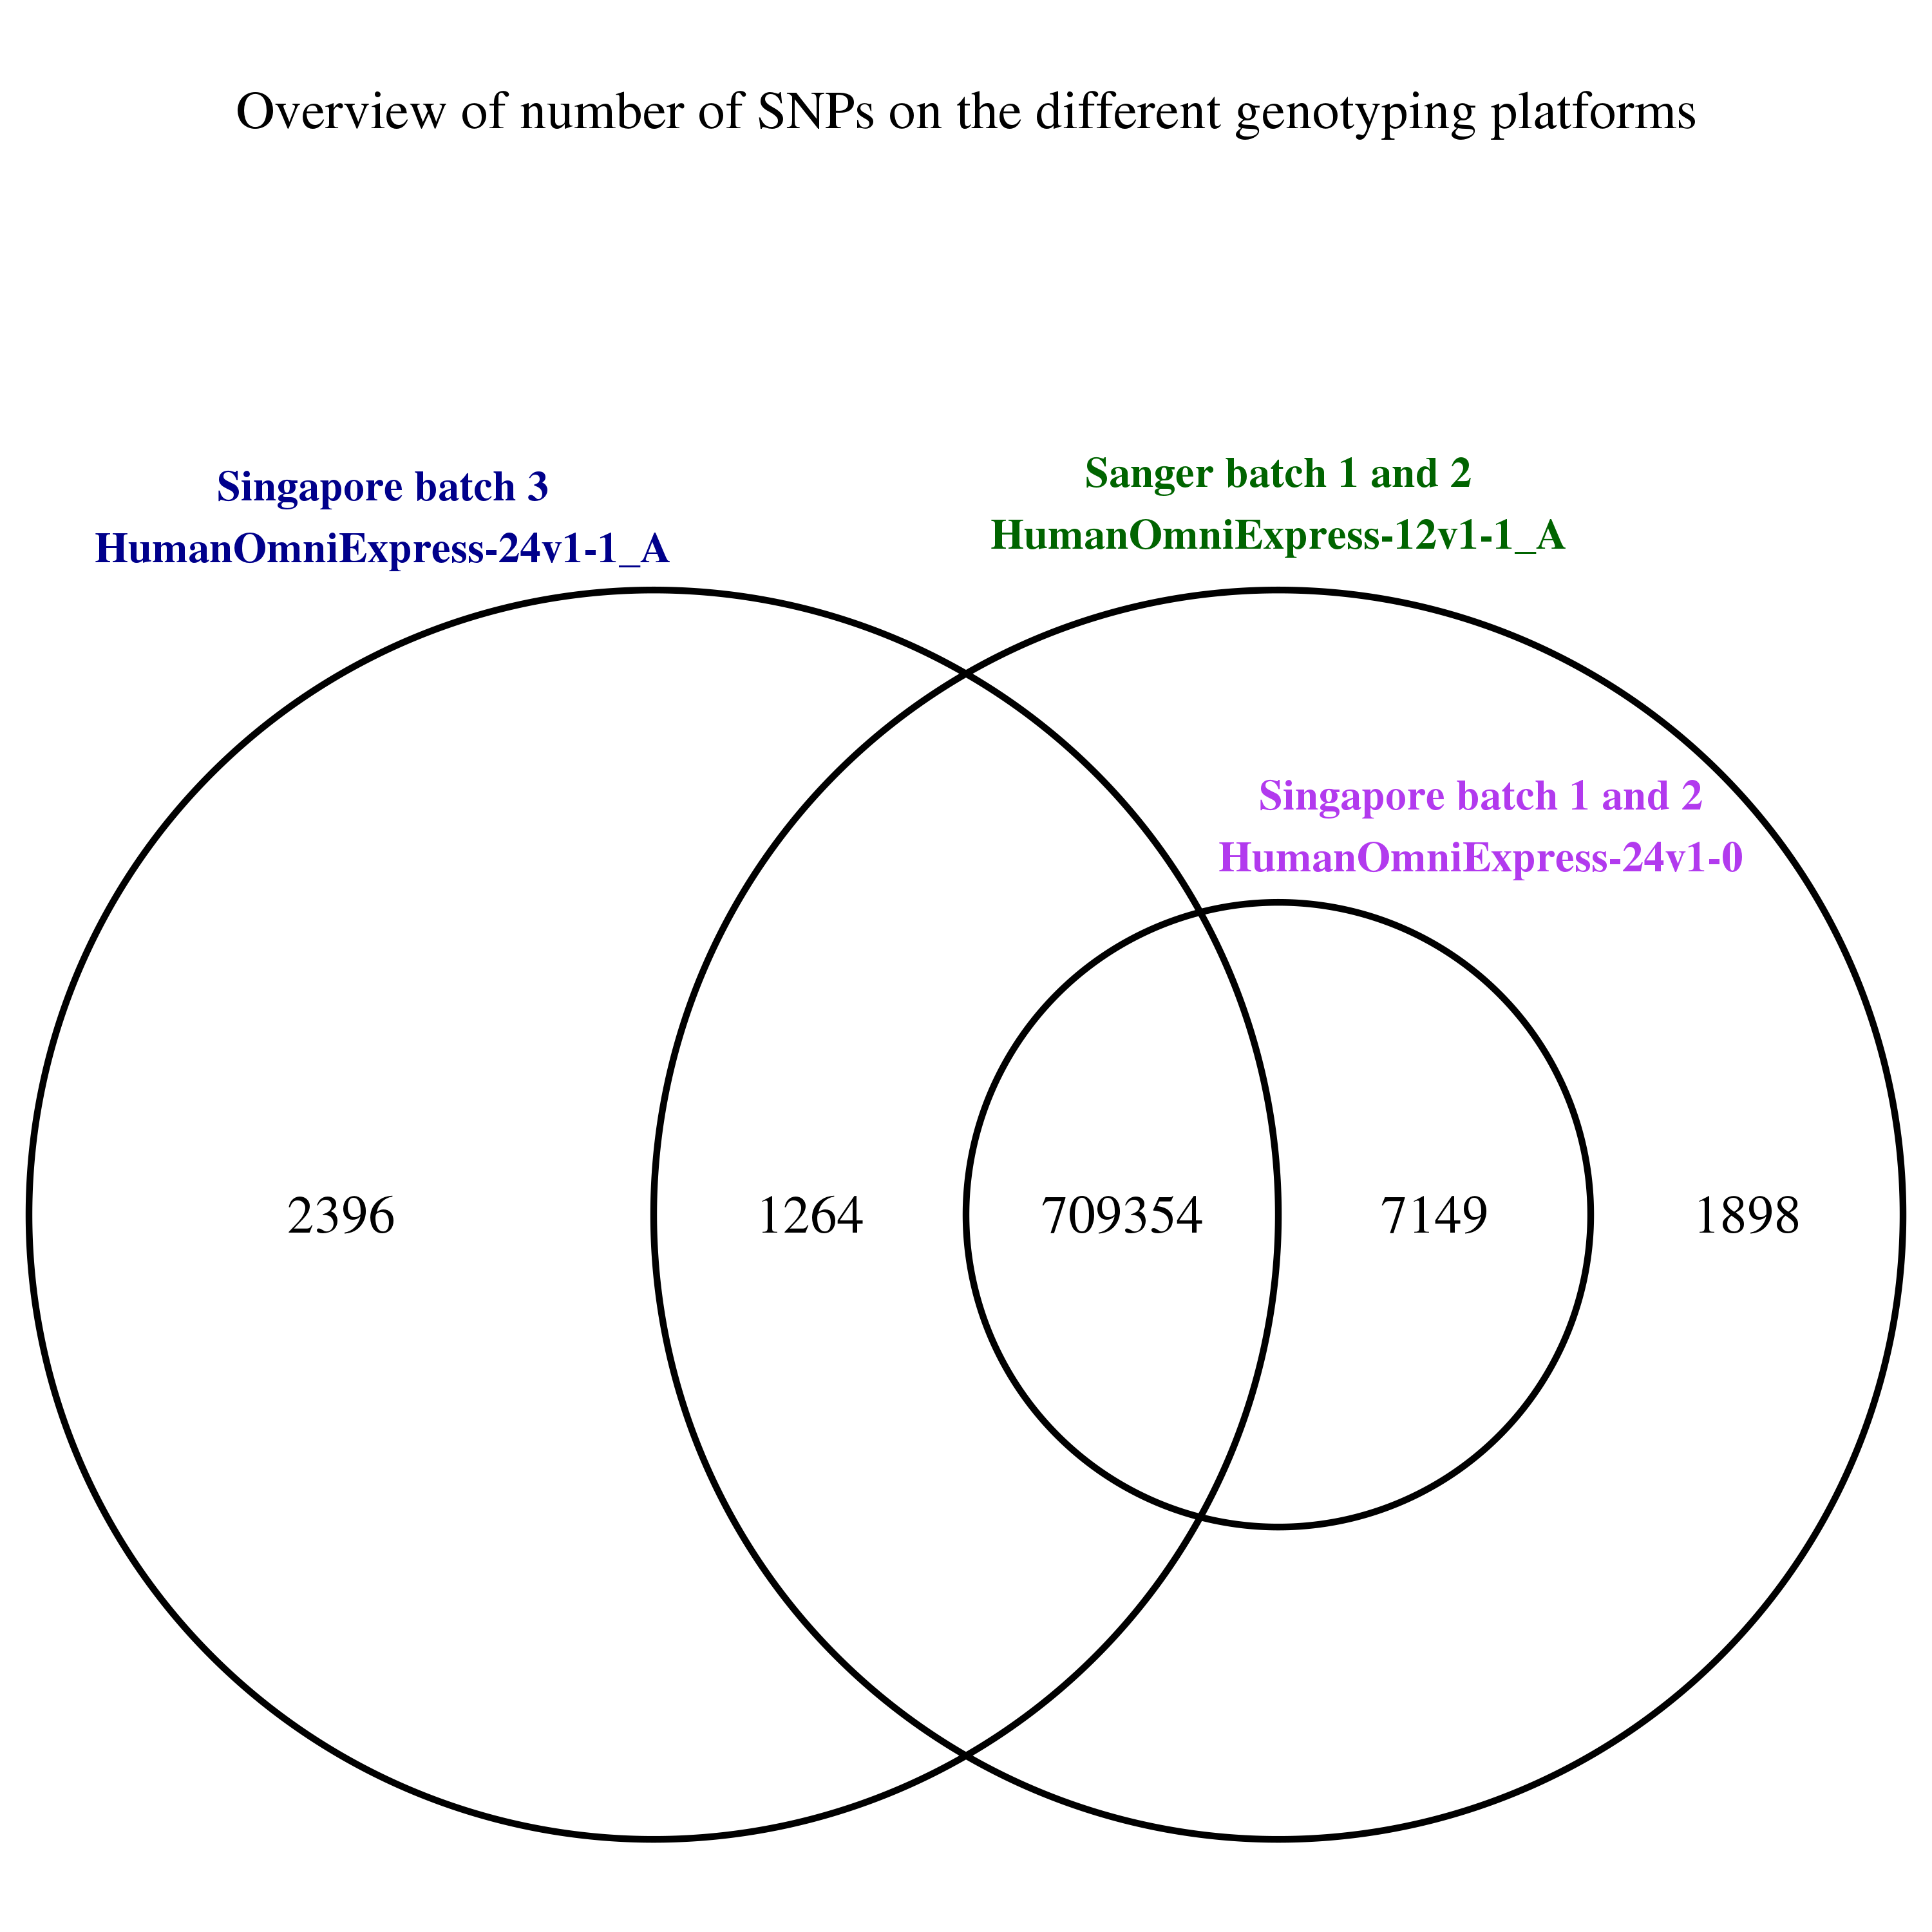
\includegraphics[trim = 0mm 0mm 0mm 20mm, clip, width=0.9\textwidth]{Supplement/Figures/Venn_genotyping_batches.pdf}
	\caption[\textbf{Number of DNA probes on the different genotyping chips and their overlap.}]{\textbf{Number of DNA probes on the different genotyping chips and their overlap.} For the genotyping of the individuals in the Digital Heart project three different Illumina HumanOmniExpress genotyping chips were used (24v1-1\_A, 12v1-1\_A, 24v1-0), differing in the number of probes on the chip (numbers inside Venn diagram) and the number of samples that can be genotyped (12 and 24; indicated in name of chip).}
 	\label{fig:probeoverlap}
\end{figure}

\begin{figure}[hbtp]
	\centering
	\includegraphics[trim = 0mm 0mm 0mm 0mm, clip, width=\textwidth]{Supplement/Figures/SampleQC.pdf}
	\caption[\textbf{Genotyping quality control per sample.}]{\textbf{Genotyping quality control per sample.} A. Sanger12. B. Duke-NUS12. C. Duke-NUS3. Supplementary plots for genotyping QC described in \cref{subsection:genotypes}.}
 	\label{fig:sampleQC}
\end{figure}

\begin{figure}[hbtp]
	\centering
	\includegraphics[trim = 0mm 0mm 0mm 0mm, clip, width=\textwidth]{Supplement/Figures/SNPQC.pdf}
	\caption[\textbf{Genotyping quality control per SNP.}]{\textbf{Genotyping quality control per SNP.} A. Sanger12. B. Duke-NUS12. C. Duke-NUS3. Supplementary plots for genotyping QC described in \cref{subsection:genotypes}.}
 	\label{fig:SNPQC}
 	\end{figure}

\begin{figure}[hbtp]
	\centering
	\includegraphics[trim = 0mm 0mm 0mm 0mm, clip,  width=\textwidth]{Supplement/Figures/kinshipQC.pdf}
	\caption[\textbf{Ethnicity of samples within the Digitial Heart project. }]{\textbf{Ethnicity of samples within the Digitial Heart project.} A. Sanger12. B. Duke-NUS12. C. Duke-NUS3. PCA was conducted on the SNP genotypes of the samples within the Digitial Heart project (gencall) and genotypes of four greater ethnicities of the HapMap project (black: African, orange:Mexican/Native American, grey: Caucasian, yellow: Asian) \citep{HapMap2003,HapMap2005}. The clustering of the samples based on the first and second principal components are depicted. Red dotted lines indicate borders considered to separate ethnicities: 1. Caucasian, 2: African, 3: Mexican/Native American, 4. Asian, 5: Mixed ancestry. Gencall samples within the first group were used in \cref{chapter:GWAS-3Dheart,chapter:GWAS-FD}.  A descriptionof the analysis is described in \cref{subsection:genotypes}.}
 	\label{fig:kinshipQC}
\end{figure}

\newpage
\section{Imputation}

% Table generated by Excel2LaTeX from sheet 'imputationQC'
\begin{table}[htbp]
  \centering
  \caption[\textbf{Number of SNPs after imputation, imputation QC and filtering for deviation from HWE and low MAF. }]{\textbf{Number of SNPs after imputation, imputation QC and filtering for deviation from HWE and low MAF. } Every batch was imputed independently (columns `SNPs after imputation'). SNPs that had an IMPUTE2 `info' metric of \(> 0.4\) in all of the batches were combined and subsequently filtered for SNPs deviating from HWE (\(p <0.001\)) and with low MAF (\(< 0.008\)), corresponding to a MAC of less than \num{20}. }
    \begin{tabular}{llllll}
    \toprule
    \multicolumn{1}{c}{\multirow{2}[4]{*}{Chr}} & \multicolumn{3}{c}{SNPs after Imputation} & \multicolumn{1}{c}{\multirow{2}[4]{*}{ INFO > 0.4}} & \multicolumn{1}{c}{\multirow{2}[4]{*}{HWE and MAF}} \\
\cmidrule{2-4}          & Sanger12 & Duke-NUS12 & Duke-NUS3 &       &  \\
    \midrule
    \num{1} & \num{3196692} & \num{3197145} & \num{3196563} & \num{1251157} & \num{719882} \\
    \num{2} & \num{3515670} & \num{3515861} & \num{3515602} & \num{1360182} & \num{780152} \\
    \num{3} & \num{2941265} & \num{2941468} & \num{2941223} & \num{1156243} & \num{665038} \\
    \num{4} & \num{2900679} & \num{2900786} & \num{2900634} & \num{1154742} & \num{684602} \\
    \num{5} & \num{2688219} & \num{2688348} & \num{2688174} & \num{1049671} & \num{606951} \\
    \num{6} & \num{2581500} & \num{2581851} & \num{2581410} & \num{1058844} & \num{635257} \\
    \num{7} & \num{2359370} & \num{2359598} & \num{2359319} & \num{932726} & \num{551744} \\
    \num{8} & \num{2323181} & \num{2323290} & \num{2323144} & \num{890407} & \num{514803} \\
    \num{9} & \num{1752242} & \num{1752363} & \num{1752199} & \num{698510} & \num{398777} \\
    \num{10} & \num{2003743} & \num{2003881} & \num{2003694} & \num{812616} & \num{474686} \\
    \num{11} & \num{2013331} & \num{2013535} & \num{2013273} & \num{794587} & \num{481479} \\
    \num{12} & \num{1947915} & \num{1948107} & \num{1947865} & \num{767854} & \num{452193} \\
    \num{13} & \num{1458325} & \num{1458401} & \num{1458308} & \num{590863} & \num{348525} \\
    \num{14} & \num{1333919} & \num{1333973} & \num{1333901} & \num{524391} & \num{309825} \\
    \num{15} & \num{1194294} & \num{1194406} & \num{1194264} & \num{458617} & \num{266813} \\
    \num{16} & \num{1289127} & \num{1289335} & \num{1289074} & \num{497688} & \num{286620} \\
    \num{17} & \num{1118587} & \num{1118772} & \num{1118528} & \num{434724} & \num{252227} \\
    \num{18} & \num{1153963} & \num{1154034} & \num{1153942} & \num{457454} & \num{268986} \\
    \num{19} & \num{877689} & \num{877866} & \num{877645} & \num{361419} & \num{222264} \\
    \num{20} & \num{912602} & \num{912721} & \num{912574} & \num{357156} & \num{210128} \\
    \num{21} & \num{546390} & \num{546414} & \num{546381} & \num{216911} & \num{131079} \\
    \num{22} & \num{531437} & \num{531528} & \num{531416} & \num{215547} & \num{129771} \\
    \midrule
    genome & \num{42989377} & \num{42993178} & \num{42988308} & \num{16042309} & \num{9391802} \\
    \bottomrule
    \end{tabular}%
  \label{tab:imputationQC}%
\end{table}%

\newpage
\section{Dimensionality reduction}
\begin{figure}[hbtp]
	\centering
	\includegraphics[trim = 0mm 0mm 0mm 0mm, clip, width=0.65\textwidth]{Supplement/Figures/distributionAll-DimRed.pdf}
	\caption[\textbf{Additional scatterplots for visual assessement of low-dimensional components derived from left-ventricular wall thickness. }]{\textbf{Additional scatterplots for visual assessement of low-dimensional components derived from left-ventricular wall thickness. }Pairwise scatter plots of the components (lower triangle) and density plots (upper triangle) are depicted. The diagonal of each plot shows the distribution of the respective component. Row and colum labels specify the rank of the component out of the \num{100} low-dimensional components. Before plotting, each component was mean-centered and divided by its standard deviation in order to have comparable axis dimensions. Given the normalised scale of the data, and the purpose of qualitative comparison, axis ticks were omitted for a cleaner visualisation. }
	 	\label{fig:distributionAll-DimRed}
\end{figure}

\newpage
\chapter{Additional LiMMBo results}
\begin{figure}[hbtp]
	\centering
	\includegraphics[trim = 0mm 0mm 0mm 0mm, clip, width=\textwidth]{Supplement/Figures/powerAll.pdf}
		\caption[\textbf{All parameter combinations of power comparison for mvLMM and uvLMMs of high-dimensional phenotypes.}]{\textbf{All parameter combinations of power comparison for mvLMM and uvLMMs of high-dimensional phenotypes.} Each panels show the influence of one simulation parameter on the power to detect the causal SNPs.} 
	 	\label{fig:power-all}
\end{figure}


\newpage
\chapter{Additional GWAS results}
\begin{figure}[hbtp]
	\centering
	\includegraphics[trim = 0mm 0mm 0mm 0mm, clip, width=0.65\textwidth]{Supplement/Figures/manhattan-all.pdf}
	\caption[\textbf{Manhattan plots for GWAS on stable components from a single dimensionality reduction method. }]{\textbf{Manhattan plots for GWAS on stable components from a single dimensionality reduction method. }The five stable components derived from Laplacian Eigenmaps (A), four from Isomap (B) and ten from PCA (C) were used as the response variables in three independent any effect multi-trait GWAS. Their p-values were adjusted for the effective number of test conducted, estimated via \cref{eq:meff} based on the correlation across their components (\cref{fig:dimRed-correlation}): \(M_{eff}=2.04\). The horizontal grey line is drawn at the level of genome-wide significance: \(p = 5 \times 10^{-8}\). Only the locus on chromosome 1 which was detected in the combined analyses (\cref{fig:manhattan-heart}) could also be detected via components from Laplacian Eigenmaps alone. } 
	 	\label{fig:manhattan-3Dheart-single}
\end{figure}


\begin{figure}[hbtp]
	\centering
	\includegraphics[trim = 0mm 0mm 0mm 0mm, clip, width=0.65\textwidth]{Supplement/Figures/manhattan-FD-single.pdf}
	\caption[\textbf{Manhattan plot of  two single-trait GWAS on left ventricular trabeculation. }]{\textbf{Manhattan plot of two single-trait GWAS on left ventricular trabeculation } The maximal apical (A) and basal FD (B) were used as the response variable in a single-trait GWAS.  Their p-values were adjusted for the effective number of test conducted, estimated via \cref{eq:meff} based on their correlation: \(M_{eff}=1.86\). The p-values of all genome-wide SNPs are depicted. The horizontal grey line is drawn at the level of genome-wide significance: \(p = 5 \times 10^{-8}\).} 
	 	\label{fig:manhattan-FD-single}
\end{figure}